\subsubsection{Resource Decryption} \label{subsection:counter-replace-encryption-content-resource}
The first approach is to apply encryption on the application's static resources.
This includes the application's hard coded strings as well as image assets.
Whenever a resource is used, it has to be decrypted first.
The increase in security comes at the cost of decreased performance.
As long as application critical strings, like server addresses are encrypted, the application is unable to work.
In case no critical strings are present, the application will work as usual, but the user experience will be not sufficient because all strings are still encrypted and thus have no meaning.
Figure~\ref{fig:encryptionResource} shows the abstract implementation of resource decryption.
\begin{figure}[h]
    \centering
    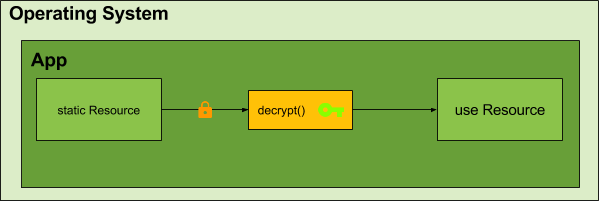
\includegraphics[width=0.8\textwidth]{data/encryptionResource.png}
    \caption{Encrypted resources which have to be decrypted on startup}
    \label{fig:encryptionResource}
\end{figure}
